\documentclass{ximera}

 

\usepackage{epsfig}

\graphicspath{
  {./}
  {figures/}
}

\usepackage{morewrites}
\makeatletter
\newcommand\subfile[1]{%
\renewcommand{\input}[1]{}%
\begingroup\skip@preamble\otherinput{#1}\endgroup\par\vspace{\topsep}
\let\input\otherinput}
\makeatother

\newcommand{\includeexercises}{\directlua{dofile("/home/jim/linearAlgebra/laode/exercises.lua")}}

%\newcounter{ccounter}
%\setcounter{ccounter}{1}
%\newcommand{\Chapter}[1]{\setcounter{chapter}{\arabic{ccounter}}\chapter{#1}\addtocounter{ccounter}{1}}

%\newcommand{\section}[1]{\section{#1}\setcounter{thm}{0}\setcounter{equation}{0}}

%\renewcommand{\theequation}{\arabic{chapter}.\arabic{section}.\arabic{equation}}
%\renewcommand{\thefigure}{\arabic{chapter}.\arabic{figure}}
%\renewcommand{\thetable}{\arabic{chapter}.\arabic{table}}

%\newcommand{\Sec}[2]{\section{#1}\markright{\arabic{ccounter}.\arabic{section}.#2}\setcounter{equation}{0}\setcounter{thm}{0}\setcounter{figure}{0}}

\newcommand{\Sec}[2]{\section{#1}}

\setcounter{secnumdepth}{2}
%\setcounter{secnumdepth}{1} 

%\newcounter{THM}
%\renewcommand{\theTHM}{\arabic{chapter}.\arabic{section}}

\newcommand{\trademark}{{R\!\!\!\!\!\bigcirc}}
%\newtheorem{exercise}{}

\newcommand{\dfield}{{\sf dfield9}}
\newcommand{\pplane}{{\sf pplane9}}

\newcommand{\EXER}{\section*{Exercises}}%\vspace*{0.2in}\hrule\small\setcounter{exercise}{0}}
\newcommand{\CEXER}{}%\vspace{0.08in}\begin{center}Computer Exercises\end{center}}
\newcommand{\TEXER}{} %\vspace{0.08in}\begin{center}Hand Exercises\end{center}}
\newcommand{\AEXER}{} %\vspace{0.08in}\begin{center}Hand Exercises\end{center}}

% BADBAD: \newcommand{\Bbb}{\bf}

\newcommand{\R}{\mbox{$\Bbb{R}$}}
\newcommand{\C}{\mbox{$\Bbb{C}$}}
\newcommand{\Z}{\mbox{$\Bbb{Z}$}}
\newcommand{\N}{\mbox{$\Bbb{N}$}}
\newcommand{\D}{\mbox{{\bf D}}}
\usepackage{amssymb}
%\newcommand{\qed}{\hfill\mbox{\raggedright$\square$} \vspace{1ex}}
%\newcommand{\proof}{\noindent {\bf Proof:} \hspace{0.1in}}

\newcommand{\setmin}{\;\mbox{--}\;}
\newcommand{\Matlab}{{M\small{AT\-LAB}} }
\newcommand{\Matlabp}{{M\small{AT\-LAB}}}
\newcommand{\computer}{\Matlab Instructions}
\newcommand{\half}{\mbox{$\frac{1}{2}$}}
\newcommand{\compose}{\raisebox{.15ex}{\mbox{{\scriptsize$\circ$}}}}
\newcommand{\AND}{\quad\mbox{and}\quad}
\newcommand{\vect}[2]{\left(\begin{array}{c} #1_1 \\ \vdots \\
 #1_{#2}\end{array}\right)}
\newcommand{\mattwo}[4]{\left(\begin{array}{rr} #1 & #2\\ #3
&#4\end{array}\right)}
\newcommand{\mattwoc}[4]{\left(\begin{array}{cc} #1 & #2\\ #3
&#4\end{array}\right)}
\newcommand{\vectwo}[2]{\left(\begin{array}{r} #1 \\ #2\end{array}\right)}
\newcommand{\vectwoc}[2]{\left(\begin{array}{c} #1 \\ #2\end{array}\right)}

\newcommand{\ignore}[1]{}


\newcommand{\inv}{^{-1}}
\newcommand{\CC}{{\cal C}}
\newcommand{\CCone}{\CC^1}
\newcommand{\Span}{{\rm span}}
\newcommand{\rank}{{\rm rank}}
\newcommand{\trace}{{\rm tr}}
\newcommand{\RE}{{\rm Re}}
\newcommand{\IM}{{\rm Im}}
\newcommand{\nulls}{{\rm null\;space}}

\newcommand{\dps}{\displaystyle}
\newcommand{\arraystart}{\renewcommand{\arraystretch}{1.8}}
\newcommand{\arrayfinish}{\renewcommand{\arraystretch}{1.2}}
\newcommand{\Start}[1]{\vspace{0.08in}\noindent {\bf Section~\ref{#1}}}
\newcommand{\exer}[1]{\noindent {\bf \ref{#1}}}
\newcommand{\ans}{}
\newcommand{\matthree}[9]{\left(\begin{array}{rrr} #1 & #2 & #3 \\ #4 & #5 & #6
\\ #7 & #8 & #9\end{array}\right)}
\newcommand{\cvectwo}[2]{\left(\begin{array}{c} #1 \\ #2\end{array}\right)}
\newcommand{\cmatthree}[9]{\left(\begin{array}{ccc} #1 & #2 & #3 \\ #4 & #5 &
#6 \\ #7 & #8 & #9\end{array}\right)}
\newcommand{\vecthree}[3]{\left(\begin{array}{r} #1 \\ #2 \\
#3\end{array}\right)}
\newcommand{\cvecthree}[3]{\left(\begin{array}{c} #1 \\ #2 \\
#3\end{array}\right)}
\newcommand{\cmattwo}[4]{\left(\begin{array}{cc} #1 & #2\\ #3
&#4\end{array}\right)}

\newcommand{\Matrix}[1]{\ensuremath{\left(\begin{array}{rrrrrrrrrrrrrrrrrr} #1 \end{array}\right)}}

\newcommand{\Matrixc}[1]{\ensuremath{\left(\begin{array}{cccccccccccc} #1 \end{array}\right)}}



\renewcommand{\labelenumi}{\theenumi)}
\newenvironment{enumeratea}%
{\begingroup
 \renewcommand{\theenumi}{\alph{enumi}}
 \renewcommand{\labelenumi}{(\theenumi)}
 \begin{enumerate}}
 {\end{enumerate}\endgroup}



\newcounter{help}
\renewcommand{\thehelp}{\thesection.\arabic{equation}}

%\newenvironment{equation*}%
%{\renewcommand\endequation{\eqno (\theequation)* $$}%
%   \begin{equation}}%
%   {\end{equation}\renewcommand\endequation{\eqno \@eqnnum
%$$\global\@ignoretrue}}

%\input{psfig.tex}

\author{Martin Golubitsky and Michael Dellnitz}

%\newenvironment{matlabEquation}%
%{\renewcommand\endequation{\eqno (\theequation*) $$}%
%   \begin{equation}}%
%   {\end{equation}\renewcommand\endequation{\eqno \@eqnnum
% $$\global\@ignoretrue}}

\newcommand{\soln}{\textbf{Solution:} }
\newcommand{\exercap}[1]{\centerline{Figure~\ref{#1}}}
\newcommand{\exercaptwo}[1]{\centerline{Figure~\ref{#1}a\hspace{2.1in}
Figure~\ref{#1}b}}
\newcommand{\exercapthree}[1]{\centerline{Figure~\ref{#1}a\hspace{1.2in}
Figure~\ref{#1}b\hspace{1.2in}Figure~\ref{#1}c}}
\newcommand{\para}{\hspace{0.4in}}

\renewenvironment{solution}{\suppress}{\endsuppress}

\ifxake
\newenvironment{matlabEquation}{\begin{equation}}{\end{equation}}
\else
\newenvironment{matlabEquation}%
{\let\oldtheequation\theequation\renewcommand{\theequation}{\oldtheequation*}\begin{equation}}%
  {\end{equation}\let\theequation\oldtheequation}
\fi

\makeatother


\title{Saddle-Node Bifurcations Revisited}

\begin{document}
\begin{abstract}
\end{abstract}
\maketitle


\label{S:SNB}
\index{bifurcation!steady-state}  \index{bifurcation!saddle-node}


The simplest steady-state bifurcations --- and the ones that are most
likely to occur --- are the saddle-node bifurcations.  In 
Section~\ref{S:bifurcation} we found necessary conditions for the existence 
of saddle-node bifurcations in one dimension \Ref{E:DCSN} and two 
dimensions \Ref{E:DCSN2}.  In this section we describe necessary and 
sufficient conditions for the existence of saddle-node bifurcations.


\subsection*{Saddle-Node Bifurcation in One Dimension}

Consider the differential equation 
\begin{equation} \label{e:1dbif}
\dot{x} = f(x,\rho),
\end{equation}
that depends on the single parameter $\rho$.  The equilibria are 
found by solving the algebraic equation 
\begin{equation} \label{e:1dstst}
f(x,\rho) = 0.
\end{equation}
We can study how the equilibria in phase portraits for \Ref{e:1dbif} 
change when $\rho$ is varied by plotting
solutions to \Ref{e:1dstst} in the $\rho x$-plane.  The solutions to
\Ref{e:1dstst} form the bifurcation diagram of \Ref{e:1dbif}.

Recall from \Ref{E:DCSN} that  
\begin{equation}  \label{e:1dbifcond}
\begin{array}{rcl}
f(x_0,\rho_0) & = & 0 \\
f_x(x_0,\rho_0) & = & 0.
\end{array}
\end{equation}
are necessary conditions for a saddle-node bifurcation to occur at
$(x_0,\rho_0)$.  The simplest example of a saddle-node bifurcation is:
\begin{equation}  \label{e:1dsaddlenf}
f(x,\rho) = a x^2 + \rho,
\end{equation}
where $a$ is a nonzero constant.  The exact bifurcation diagram for 
\Ref{e:1dsaddlenf} depends on the sign of $a$.  See Figure~\ref{F:1dsaddle}.  
Note that the bifurcation diagram is just a parabola pointing either to the 
left or to the right.  The general saddle-node bifurcation is one whose 
bifurcation diagram looks `parabolic-like'.  Theorem~\ref{T:saddlenode}
makes this idea precise.

\begin{figure}[htb]
           \centerline{%
	   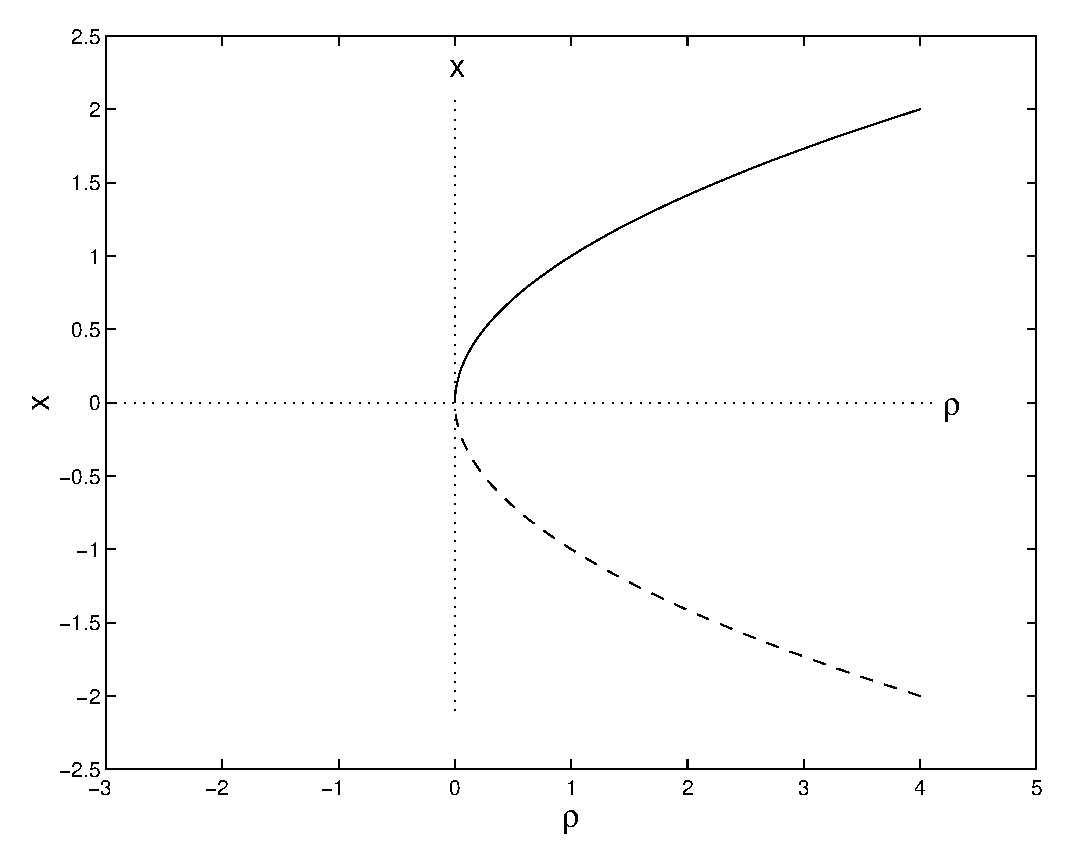
\psfig{file=../figures/sbifBIF.eps,width=2.5in} \qquad \qquad
	   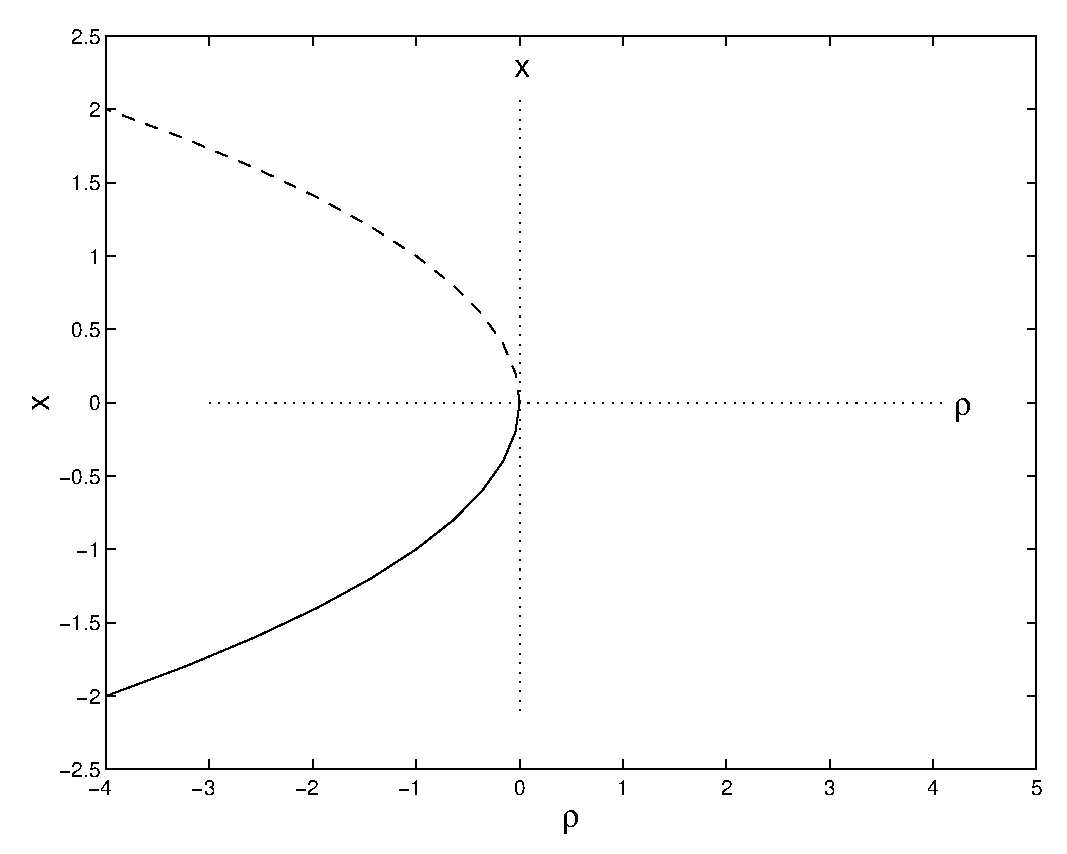
\psfig{file=../figures/sbifBIF2.eps,width=2.5in}}
	 \hspace{1.0in} $a<0$ \hspace{2.8in}  $a>0$  
           \caption{Bifurcation diagrams for \protect\Ref{e:1dsaddlenf}.}
           \label{F:1dsaddle}
\end{figure}

\begin{theorem}  \label{T:saddlenode} \index{bifurcation!saddle-node}
Suppose that the differential equation \Ref{e:1dbif} has an equilibrium
at $(x_0,\rho_0)$ satisfying the bifurcation conditions \Ref{e:1dbifcond}
and the nondegeneracy conditions\index{nondegeneracy conditions}
\begin{equation}  \label{e:nondegen1}
\begin{array}{rcl} 
f_\rho(x_0,\rho_0) & \neq & 0 \\
f_{xx}(x_0,\rho_0) & \neq & 0. 
\end{array}
\end{equation}
Then the bifurcation diagram $f=0$ looks like the diagram in 
Figure~\ref{F:1dsaddle} where 
\[
a = \frac{f_{xx}(x_0,\rho_0)}{f_\rho(x_0,\rho_0)}.
\]
\end{theorem}

\begin{proof}  The proof of this theorem uses the implicit function theorem and
implicit differentiation.  (Technically, we need to assume that the second
derivatives of $f(x,\rho)$ are continuous before proceeding.) Since 
$f_\rho(x_0,\rho_0)$ is assumed to be nonzero, the implicit function theorem 
guarantees the existence of a function $R(x)$ such that $R(x_0)=\rho_0$ and
\begin{equation}  \label{e:implicit0}
f(x,R(x))\equiv 0
\end{equation}
for all $x$ near $x_0$.  It follows that the bifurcation diagram $f(x,\rho)=0$
is the graph $\rho = R(x)$.  We claim that $R'(x_0)=0$ and $R''(x_0)\neq 0$. 
Thus the Taylor series of the function $R(x)$ is
\[
R(x) = \rho_0 + \half R''(x_0)(x-x_0)^2 + \cdots 
\]
for all $x$ near $x_0$.  It follows that the bifurcation diagram $f=0$ is
parabolic in shape as in Figure~\ref{F:1dsaddle} --- opening either to the 
left or to the right depending on the sign of $R''(x_0)$.

We use implicit differentiation to verify these claims. Differentiating
\Ref{e:implicit0} twice yields 
\begin{equation}  \label{e:implicit1}
f_x(x,R(x)) + f_\rho(x,R(x))R'(x) \equiv 0,
\end{equation}
and 
\begin{equation}  \label{e:implicit2}
f_{xx}(x,R(x)) + 2f_{x\rho}(x,R(x))R'(x) + f_{\rho\rho}(x,R(x))R'(x)^2 
+ f_\rho(x,R(x))R''(x) \equiv 0.
\end{equation}

Evaluating \Ref{e:implicit1} at $x=x_0$ yields
\[
f_x(x_0,\rho_0) + f_\rho(x_0,\rho_0)R'(x_0) = 0. 
\]
Since, by assumption, $f_x(x_0,\rho_0)=0$ and $f_\rho(x_0,\rho_0)\neq 0$,
it follows that 
\[
R'(x_0)=0.
\]
Evaluating \Ref{e:implicit2} at $x=x_0$ now yields
\[
f_{xx}(x_0,\rho_0) +  f_\rho(x_0,\rho_0)R''(x_0) = 0
\]
The nondegeneracy assumptions \Ref{e:nondegen1} imply
\[
R''(x_0) = -\frac{f_{xx}(x_0,\rho_0)}{f_\rho(x_0,\rho_0)} \neq 0.
\]
Thus $a=-R''(x_0)$.  So when $R''(x_0)>0$ the number $a$ is negative and the
bifurcating branch is supercritical, as in Figure~\ref{F:1dsaddle}.  Similarly, 
when $R''(x_0)<0$ the number $a$ is positive and the bifurcating branch is 
subcritical. \end{proof}
 
\subsubsection*{An Example of a One Dimensional Saddle-Node Bifurcation}

Consider the following example of a saddle-node bifurcation.  Let 
\begin{equation}  \label{e:sn1}
f(x,\rho) = -x^3 + 3x^2 - \rho x - 4.
\end{equation}
A quick check shows that $x=2$ is an equilibrium for \Ref{e:sn1} 
when $\rho=0$.  Moreover, 
\[
f(2,0)=0, \quad f_x(2,0)=0, \quad f_\rho(2,0)=-2\neq 0, 
\quad f_{xx}(2,0)=-6\neq 0.
\]
It follows from Theorem~\ref{T:saddlenode} that $f$ has a saddle-node
bifurcation when $\rho=0$ at $x=2$.  Indeed, since $a=\frac{-6}{-2}=3>0$, 
it follows that there are two equilibria near $x=2$ when $\rho<0$ and 
none when $\rho>0$.  See Figure~\ref{F:1dsaddle}. This fact can be 
verified using {\sf pline}.  When $\rho$ is small and positive, there is 
one stable equilibrium near $x=-1$.  When $\rho$ is small and negative, there 
are three equilibria --- the stable one near $x=-1$ and two new equilibria 
near $x=2$ formed from the saddle-node bifurcation.  



\subsection*{Saddle-Node Bifurcations in Two Dimensions}
\index{bifurcation!saddle-node}

In higher dimensions, steady-state bifurcations occur at parameter 
values where the Jacobian matrix\index{matrix!Jacobian}
has a zero eigenvalue.  In one dimension,
the $1\times 1$ Jacobian matrix is the number $f_x$.  Such a 
Jacobian matrix has a zero eigenvalue precisely when $f_x$ vanishes
--- which is just the condition in \Ref{e:1dbifcond}.  

In two dimensions, the Jacobian matrix $J$ is a saddle-node matrix when
it has a single zero eigenvalue, that is, when $\det(J)=0$ and 
$\trace(J)\neq 0$.  Now consider the planar system of differential equations 
depending on a parameter $\rho$.  We write this system as
\begin{equation}  \label{e:2deqn}
\dot{X} = F(X,\rho),
\end{equation}
where $X=(x,y)\in\R^2$ and $F=(g,h)$ in coordinates.  Sufficient conditions
for the existence of a saddle-node bifurcation in \Ref{e:2deqn} are as follows.
\begin{enumerate}
\item Equation~\Ref{e:2deqn} has an equilibrium at $(X_0,\rho_0)$; so 
\[
F(X_0,\rho_0) = 0.
\]
\item  The Jacobian matrix 
\[
J=(dF)_{(X_0,\rho_0)}=
\mattwo{g_x(X_0,\rho_0)}{g_y(X_0,\rho_0)}{h_x(X_0,\rho_0)}{h_y(X_0,\rho_0)}.
\]
has a zero eigenvalue and a nonzero eigenvalue.  Let $w$ be a nonzero vector 
in the null space of $J^t$.  Assume
\begin{equation}  \label{e:2deig}
w \cdot F_\rho(X_0,\rho_0) \neq 0,
\end{equation}
where $F_\rho=(g_\rho,h_\rho)$.  (In one dimension, \Ref{e:2deig} just states 
that $f_\rho(X_0,\rho_0)$ is nonzero; that is, the first
nondegeneracy condition\index{nondegeneracy conditions} in 
\Ref{e:nondegen1} is valid.) 
\item   Let $v=(v_1,v_2)$ be a nonzero vector in the null space of $J$.
The following is an analogue in two dimensions for the second nondegeneracy
condition in \Ref{e:nondegen1}, $f_{xx}(x_0,\rho_0)\neq 0$. Define $F_0$ to 
be the vector
\[
F_0 = v_1^2\vectwo{g_{xx}}{h_{xx}} + 2v_1v_2\vectwo{g_{xy}}{h_{xy}}
+ v_2^2 \vectwo{g_{yy}}{h_{yy}}  
\]
evaluated at $(X_0,\rho_0)$.  The nondegeneracy condition in two dimensions
is:
\begin{equation}  \label{e:2dbifur}
w \cdot F_0 \neq 0.
\end{equation}
\end{enumerate}
A steady-state bifurcation is a {\em saddle-node bifurcation\/} if 
\Ref{e:2deig} and \Ref{e:2dbifur} are valid.  At a saddle-node bifurcation 
two equilibria coalesce as $\rho$ is varied, and the bifurcation diagram 
resembles that in Figure~\ref{F:1dsaddle}.

\subsubsection*{An Example of a Two Dimensional Saddle-Node Bifurcation}

As an example, consider the system of differential equations
\begin{matlabEquation}  \label{e:snex}
\begin{array}{rcccl}
\dot{x} & = & \rho + x + 3y -xy & \equiv & g(x,y) \\
\dot{y} & = & -\rho + 2x + 6y + 3x^2 & \equiv & h(x,y).  
\end{array}
\end{matlabEquation}
At $\rho = 0$, \Ref{e:snex} has an equilibrium at the origin with 
Jacobian matrix
\[
J = \mattwo{1}{3}{2}{6}.
\]
Since $\det(J)=0$, the origin is a bifurcation point.  Define the 
vectors $v$ and $w$ by
\[
Jv=0 \AND J^tw=0.
\]
So
\[
v = \vectwo{3}{-1} \AND  w = \vectwo{2}{-1}.
\]
Next compute
\[
F_\rho = \vectwo{1}{-1}.
\]
Therefore
\[
w \cdot F_\rho = \vectwo{2}{-1} \cdot \vectwo{1}{-1} = 3 \neq 0,
\]
and \Ref{e:2deig} is satisfied.  

Next compute
\[
g_{xx}=0, \quad g_{xy}=-1, \quad g_{yy}=0, \quad
h_{xx}=6, \quad h_{xy}=0, \quad h_{yy} = 0.
\]
Hence
\[
F_0 = v_1^2 \vectwo{0}{6} + 2v_1v_2\vectwo{-1}{0} = \vectwo{6}{54},
\]
and 
\[
w\cdot F_0 = \vectwo{2}{-1} \cdot \vectwo{6}{54} = -42 \neq 0.
\]
So \Ref{e:2dbifur} is satisfied. These conditions show that there is
a saddle-node bifurcation at the origin and that two equilibria 
coalesce as $\rho$ varies through zero. 

Some experimentation will convince you that it is complicated to find 
a closed form analytic solution for the equilibria of \Ref{e:snex}.  
We can, however, verify the existence of a saddle-node bifurcation 
using {\sf pplane5}.  The phase plane portraits are shown in 
Figure~\ref{F:snex}.

\begin{figure}[htb]
           \centerline{%
	   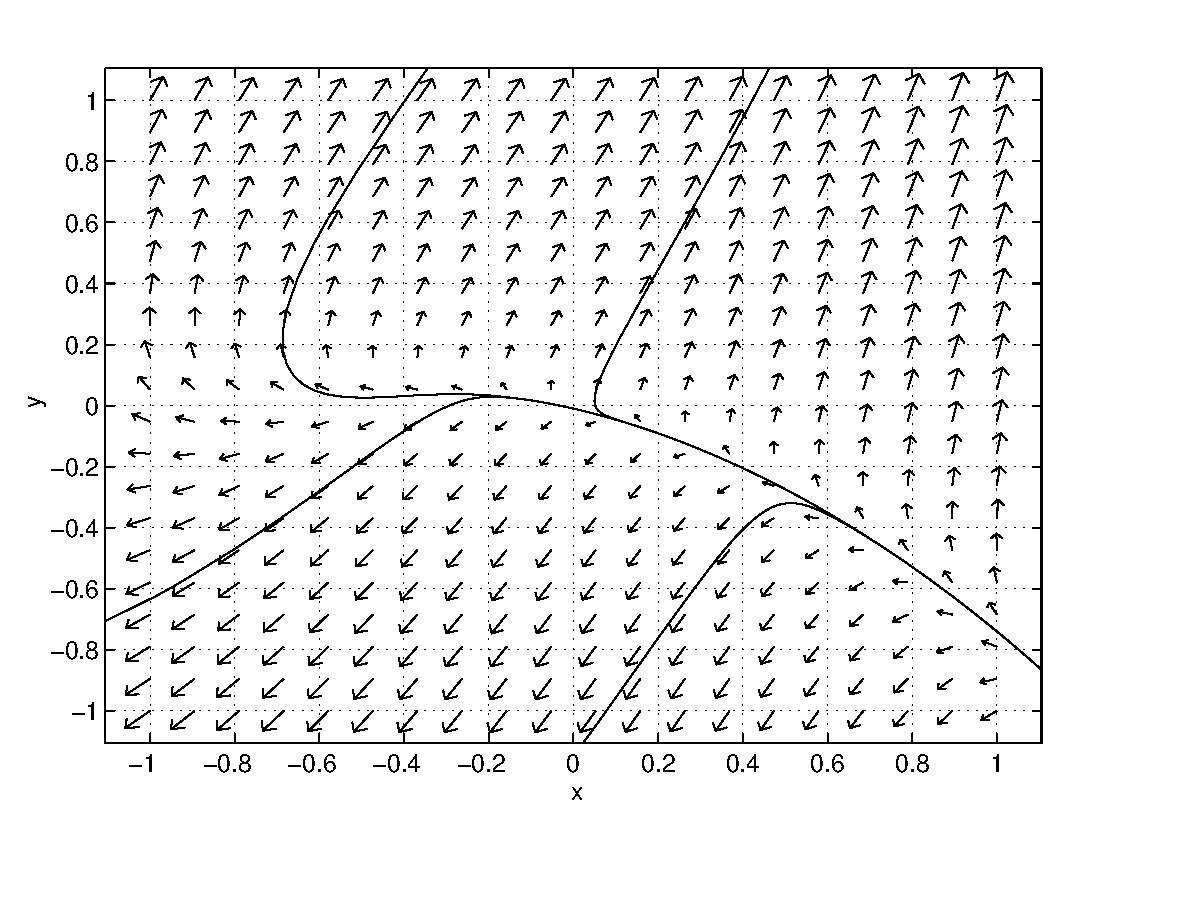
\psfig{file=../figures/snexa.eps,width=3.2in}
	   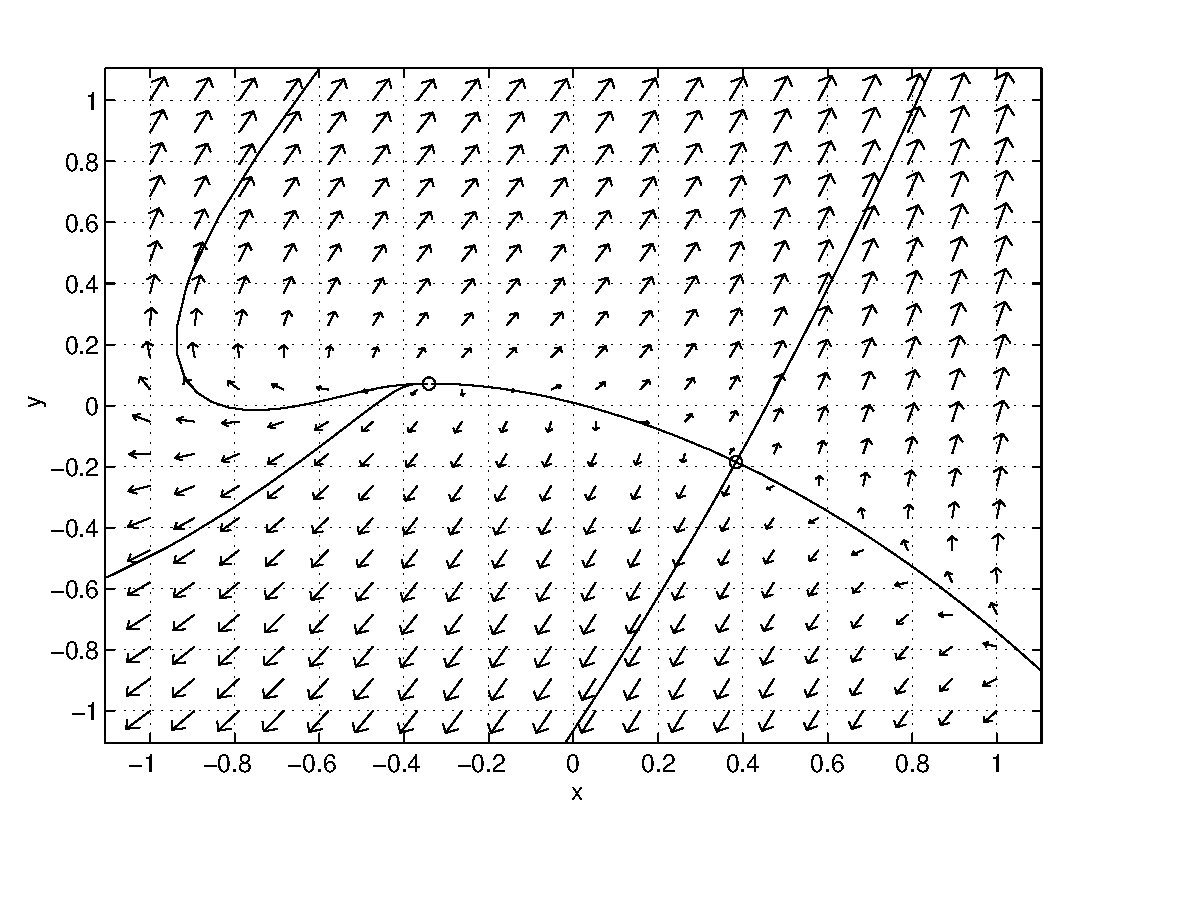
\psfig{file=../figures/snexb.eps,width=3.2in}}
	\vspace*{-0.2in}
	\hspace{1.0in} $\rho=-0.1$  \hspace{2.55in} $\rho=0.1$ 
           \caption{Phase plane portrait for \protect\Ref{e:snex} on 
	the square $-1\leq x,y \leq 1$.  Note that there are no 
	equilibria when $\rho=-0.1$ and two equilibria when $\rho=0.1$.}
           \label{F:snex}
\end{figure}


\EXER

\TEXER

\begin{exercise} \label{c9.3.1}
Let 
\begin{eqnarray*}
f_1(x,\rho) & = & \rho - x^3 \\
f_2(x,\rho) & = & \rho x - x^2.
\end{eqnarray*}
\begin{itemize}
\item[(a)] Verify that both $f_1$ and $f_2$ satisfy the bifurcation conditions 
\Ref{e:1dbifcond} at $x=0$ when $\rho=0$.
\item[(b)] Show that neither $f_1$ nor $f_2$ has a saddle-node bifurcation
at $x=0$ when $\rho=0$. 
\item[(c)] Draw the bifurcation diagrams $f_1(x,\rho)=0$ and 
$f_2(x,\rho)=0$ and explain why the conclusion of 
Theorem~\ref{T:saddlenode} is not satisfied for either $f_1$ 
or $f_2$.
\end{itemize}
\end{exercise}

\begin{exercise} \label{c9.3.5}
Find all saddle-node bifurcations in the 
family of differential equations
\begin{equation}
\dot{x} = x^3 -5x^2 + 3x + \rho
\end{equation}
analytically.  Draw the bifurcation diagram.
\end{exercise}

\begin{exercise} \label{c9.3.2}
Let 
\[
f(x,\rho) = x^4 - 6x^3 +8x^2 + 6(x-\rho) - 3.
\]
Show that $f$ has a saddle-node bifurcation at $x=3$ when $\rho=1$. 
Are there two equilibria near $x=3$ when $\rho<1$ or when $\rho>1$?
\end{exercise}

\begin{exercise} \label{c9.3.3}
Let 
\begin{eqnarray*}
g(x,y,\rho) & = &  \rho - 2x +  y + 2x^2 - y^3 \\
h(x,y,\rho) & = & 2\rho + 4x - 2y -  xy  + y^2
\end{eqnarray*}
Show that $F=(g,h)$ has a saddle-node bifurcation at $(x,y)=0$ and 
$\rho=0$.
\end{exercise}


\begin{exercise} \label{c9.3.4}
Let $X=(x,y)$ and 
\[
F(X,\rho) = \rho q + \mattwo{1}{0}{0}{0} X + Q(X)
\]
where
\[
q=\vectwo{q_1}{q_2} \AND Q(X) = \vectwo{\alpha x^2+\beta xy+\gamma y^2}
{\delta x^2 +\epsilon xy+\varphi y^2}.
\]
Show that $F$ has a saddle-node bifurcation at $X=0$ and $\rho=0$ precisely 
when $q_2\neq 0$ and $\varphi\neq 0$. 
\end{exercise}



\end{document}
